\chapter{Reflection Principle}\label{chap7}

LET\pageoriginale $(X_{t})$ BE A one-dimensional Brownian motion. Then
$P(\sup\limits_{0\leq s\leq t}X_{s}\geq a)=2P(X_{t}\geq a)$ with
$a>0$. This gives us the probability of a Brownian particle hitting
the line $x=a$ some time less than or equal to $t$. The intuitive idea
of the proof is as follows.
\begin{figure}[H]
\centering
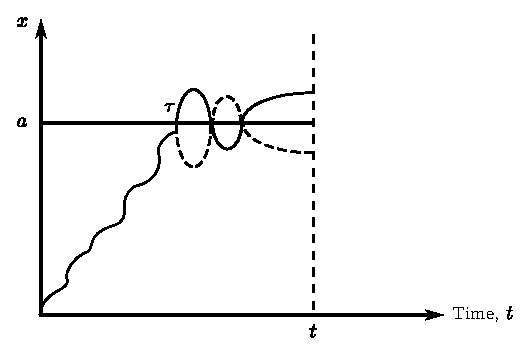
\includegraphics{figure/fig5.eps}
\end{figure}

Among all the paths that hit $a$ before time $t$ exactly half of them
end up below $a$ at time $t$. This is due to the reflection
symmetry. If $X_{s}=a$ for some $s<t$, reflection about the horizontal
line at $a$ gives a one - one correspondence between paths with
$X_{t}>a$ and paths with $X_{t}<a$. Therefore
$$
P\left\{\max\limits_{0\leq s\leq t}X_{s}\geq a,
X_{t}>a\right\}=\left\{\max\limits_{0\leq s\leq t}X_{s}\geq a, X_{t}<a\right\}
$$

Since $P\{X_{t}=a\}=0$, we obtain
\begin{align*}
P\left\{\sup\limits_{0\leq s\leq t}X_{s}\geq a\right\} &=
P\left\{\sup\limits_{0\leq s\leq t}X_{s}\geq
a,X_{t}>a\right\}+P\left\{\sup\limits_{0\leq s\leq t}X_{s}\geq
a,X_{t}>a\right\}\\
&= 2P\{X_{t}\geq a\}
\end{align*}

We\pageoriginale shall now give a precise argument. We need a few elementary
results.

\setcounter{lemma}{0}
\begin{lemma}\label{chap7-lem1}
Let $X_{n}=\sum\limits^{n}_{k=1}Y_{k}$ where the $Y_{k}$ are
independent random variables such that $P\{Y_{k}\in B\}=P\{-Y_{k}\in
B\}\forall$ Borel set $B\subset R$ (i.e. $Y_{k}$ are symmetric). Then
for any real number $a$,
$$
P\left\{\max\limits_{1\leq i\leq n} X_{i}>a\right\}\leq 2P\{X_{n}>a\}
$$
\end{lemma}

\begin{proof}
It is easy to verify that a random variable is symmetric if and only
if its characteristic function is real. Define
\begin{gather*}
A_{i}=\{X_{1}\leq a,\ldots X_{i-1}\leq a, X_{i}>a\},i=1,2,\ldots,n;\\
B=\{X_{n}>a\}
\end{gather*}

Then $A_{i}\cap A_{j}=\emptyset$ if $i\neq j$. Now,
\begin{align*}
P(A_{i}\cap B) &\geq P(A_{i}\cap \{X_{n}\geq X_{i}\})\\
&= P(A_{i})P(X_{n}\geq X_{i}),\quad\text{by independence.}\\
&= P(A_{i})P(Y_{i+1}+\cdots+Y_{n}\geq 0).
\end{align*}

As $Y_{i+1},\ldots,Y_{n}$ are independent, the characteristic function
of $Y_{i+1}+\cdots+Y_{n}$ is the product of the characteristic
functions of $Y_{i+1}+\cdots+Y_{n}$, so that $Y_{i+1}+\cdots+Y_{n}$ is
symmetric. Therefore
$$
P(Y_{i+1}+\cdots+Y_{n}\geq 0)\geq \frac{1}{2}.
$$

Thus $P(A_{i}\cap B)\geq \dfrac{1}{2}P(A_{i})$ and
$$
P(B)\geq \sum\limits^{n}_{i=1}P(A_{i}\cap B)\geq \frac{1}{2}\sum
P(A_{i})\geq \frac{1}{2}P\left(\bigcup\limits^{n}_{i=1}A_{i}\right),
$$
i.e.\pageoriginale
$$
2P(B)\geq P\left(\bigcup\limits^{n}_{i=1}A_{i}\right),
$$
or
$$
P\left\{\max\limits_{1\leq i\leq n}X_{i}>a\right\}\leq 2P\{X_{n}>a\}
$$
\end{proof}

\begin{lemma}\label{chap7-lem2}
Let $Y_{i},\ldots,Y_{n}$ be independent random variables. Put
$X_{n}=\sum\limits^{n}_{k=1}Y_{k}$ and let $\tau=\min\{i:X_{i}>a\}$,
$a>0$ and $\tau=\infty$ if there is no such $i$. Then for each
$\epsilon>0$,
\begin{itemize}
\item[\rm(a)] $P\{\tau\leq n-1,X_{n}-X_{\tau}\leq -\epsilon\}\leq
  P\{\tau\leq n-1,X_{n}\leq
  a\}+\sum\limits^{n-1}_{j=1}P(Y_{j}>\epsilon)$.

\item[\rm(b)] $P\{\tau\leq n-1,X_{n}>a+2\epsilon\}\leq P\{\tau\leq
  n-1,X_{n}-X_{\tau}>\epsilon\}+\sum\limits^{n-1}_{j=1}P\{Y_{j}>\epsilon\}$

\item[\rm(c)] $P\{X_{n}>a+2\epsilon\}\leq P\{\tau\leq n-1,X_{n}>a+2\epsilon\}+P\{Y_{n}>2\epsilon\}$.

If, further, $Y_{1},\ldots,Y_{n}$ are symmetric, then

\item[\rm(d)] $P\{\max\limits_{1\leq i\leq n}X_{i}>a,X_{n}\leq a\}\geq
  P\{X_{n}>a+2\epsilon\}-P\{Y_{n}\geq
  2\epsilon\}-2\sum\limits^{n-1}_{j=1}P\{Y_{j}>\epsilon\}$ 

\item[\rm(e)] $P\{\max\limits_{1\leq i\leq n}X_{i}>a\}\geq 2P\{X_{n}>a+2\epsilon\}-2\sum\limits^{n}_{j=1}P\{Y_{j}>\epsilon\}$
\end{itemize}
\end{lemma}

\begin{proof}
\begin{enumerate}
\renewcommand{\theenumi}{\alph{enumi}}
\renewcommand{\labelenumi}{(\theenumi)}
\item Suppose $w\in \{\tau\leq n-1,X_{n}-X_{\tau}\leq -\epsilon\}$ and
  $w\in \{\tau\leq n-1,X_{n}\leq a\}$. Then $X_{n}(w)>a$ and
  $X_{n}(w)+\epsilon\leq X_{\tau(w)}(w)$ or,
  $X_{\tau(w)}(w)>a+\epsilon$.

By definition of $\tau(w)$, $X_{\tau(w)-1}(w)\leq a$ and therefore,
$$
Y_{\tau(w)}(w)=X_{\tau(w)}(w)-X_{\tau(w)-1}(w)>a+\epsilon-a=\epsilon
$$
if $\tau(w)>1$; if $\tau(w)=1$,
$Y_{\tau(w)}(w)=X_{\tau(w)}(w)>a+\epsilon>\epsilon$. 

Thus\pageoriginale $Y_{j}(w)>\epsilon$ for some $j\leq n-1$, i.e.
$$
w\in \bigcup\limits^{n-1}_{j=1}\{Y_{j}>\epsilon\}.
$$

Therefore
$$
\{\tau\leq n-1,X_{n}-X_{\tau}\leq -\epsilon\}\subset \{\tau\leq
n-1,X_{n}\leq a\}\bigcup\limits^{n-1}_{j=1}\{Y_{j}>\epsilon\}
$$
and (q) follows.

\item Suppose $w\in \{\tau\leq n-1,X_{n}>a+2\epsilon\}$ but $w\in
  \{\tau\leq n-1,X_{n}-X_{\tau}>\epsilon\}$. Then 
$$
X_{n}(w)-X_{\tau(w)}(w)\leq \epsilon,
$$
or, $X_{\tau(w)}(w)>a+\epsilon$ so that $Y_{\tau(w)}(w)>\epsilon$ as
in (a); hence $Y_{j}(w)>\epsilon$ for some $j\leq n-1$. This proves
(b).

\item If $w\in \{X_{n}>a+2\epsilon\}$, then $\tau(w)\leq n$; if
  $w\not\in \{\tau\leq n-1,X_{n}>a+2\epsilon\}$, then $\tau(w)=n$ so
  that $X_{n-1}(w)\leq a$; therefore
  $Y_{n}(w)=X_{n}(w)-X_{n-1}(w)>2\epsilon$. i.e.\@ $w\in
  \{Y_{n}>2\epsilon\}$. Therefore
$$
\{X_{n}>a+2\epsilon\}\subset \{\tau\leq n-1,X_{n}>a+2\epsilon\}\cup\{Y_{n}>2\epsilon\}.
$$

This establishes (c).

\item \begin{tabbing}
\= $P\{\max\limits_{1\leq i\leq n}X_{i}>a,X_{n}\leq a\}=P\{\tau\leq
  n-1,X_{n}\leq a\}$\\[4pt]
\> $\geq P\{\tau\leq n-1,X_{n}-X_{\tau}\leq
-\epsilon\}-\sum\limits^{n-1}_{j=1}P(Y_{j}>\epsilon)$,\q by
(a),\\[4pt]
\> $P\left[\bigcup\limits^{n-1}_{k=1}\{\tau=k,X_{n}-X_{k}\leq
  -\epsilon\}\right]-\sum\limits^{n-1}_{j=1}P(Y_{j}>\epsilon)$\\[4pt]
\> $=\sum\limits^{n-1}_{k=1}P\{\tau=k,X_{n}-X_{k}\leq
-\epsilon\}-\sum\limits^{n-1}_{j=1}P(Y_{j}>\epsilon)$\\[4pt]
\> $=\sum\limits^{n-1}_{k=1}P\{\tau=k\}P\{X_{n}-X_{k}\leq
-\epsilon\}-\sum\limits^{n-1}_{j=1}P(Y_{j}>\epsilon)$\\[4pt]
\>\hspace{4cm} (by independence)\\[4pt]
\>
$=\sum\limits^{n}_{k=1}P\{\tau=k\}P\{X_{n}-X_{k}>\epsilon\}-\sum\limits^{n-1}_{j=1}P(Y_{j}>\epsilon)$\q
(by symmetry)\\[4pt]
\> $=P\{\tau\leq n-1,X_{n}-X_{\tau}\geq
\epsilon\}-\sum\limits^{n-1}_{j=1}P(Y_{j}>\epsilon)$\\[4pt]
\> $ \geq P\{\tau\leq
n-1,X_{n}-X_{\tau}>\epsilon\}-\sum\limits^{n-1}_{j=1}P(Y_{j}>\epsilon)$\\[4pt]
\> $\geq P\{\tau\leq
n-1,X_{n}>a+2\epsilon\}-2\sum\limits^{n-1}_{j=1}P\{Y_{j}>\epsilon\}$\q
(by (b))\\[4pt]
\> $\geq
P\{X_{n}>a+2\epsilon\}-P\{Y_{n}>2\epsilon\}-2\sum\limits^{n-1}_{j=1}P\{Y_{j}>\epsilon\}$\q
(by (c))
\end{tabbing}\pageoriginale

This proves (d).

\item \begin{tabbing}
$P\{\max\limits_{1\leq i\leq n}X_{i}>a\}$ \==
  $P\{\max\limits_{1\leq i\leq n}X_{i}>a,X_{n}\leq
  a\}+P\{\max\limits_{1\leq i\leq n}X_{i}>a,X_{n}>a\}$\\[4pt]
\>= $P\{\max\limits_{1\leq i\leq n}X_{i}>a,X_{n}\leq
a\}+P\{X_{n}>a\}$\\[4pt]
\>= $P\{X_{n}>a+2\epsilon\}-P\{Y_{n}>2\epsilon\}+P\{X_{n}>a\}$\\[4pt]
\>\hspace{2.6cm} ${}-2\sum\limits^{n-1}_{j=1}P\{Y_{j}>\epsilon\}$\q (by
(d))
\end{tabbing}

Since $P\{X_{n}>a+2\epsilon\}\leq P\{X_{n}>a\}$ and 
$$
P\{Y_{n}>2\epsilon\}\leq P\{Y_{n}>\epsilon\}\leq 2P\{Y_{n}>\epsilon\},
$$
we get
$$
P\{\max\limits_{1\leq i\leq n} X_{i}>a\}\geq
2P\{X_{n}>a+2\epsilon\}-2\sum\limits^{n}_{j=1}P(Y_{j}>\epsilon)
$$\pageoriginale 
This completes the proof.
\end{enumerate}
\end{proof}

\noindent
\textbf{\textit{Proof of the reflection principle.}}
\smallskip

By Lemma \ref{chap7-lem1}
$$
p=P\left\{\max\limits_{1\leq j\leq
  n}X\left(\frac{jt}{n}\right)>\right\}\leq 2P(X(t)>a).
$$

By Lemma \ref{chap7-lem2}(e),
$$
p\geq 2P(X(t)>a+2\epsilon)-2\sum\limits^{n}_{j=1}P\left\{\left(X\left(\frac{jt}{n}\right)-X\left(\frac{(j-1)t}{n}\right)\right)>\epsilon\right\}.
$$

Since $X\left(\dfrac{jt}{n}\right)-X\left(\dfrac{(j-1)t}{n}\right)$
are independent and 
identically distribu\-ted normal random variables with mean zero and
variance $\dfrac{t}{n}$ (in particular they are symmetric),
\begin{align*}
P\left(\left(X\left(\frac{jt}{n}\right)-X\left(\frac{(j-1)t}{n}\right)\right)>\epsilon\right)
&=
P\left(\left(X\left(\frac{t}{n}\right)-X(0)\right)>\epsilon\right)\\
&= P\left(X\left(\frac{t}{n}\right)>\epsilon\right).
\end{align*}

Therefore
$$
p\geq
2P(X(t)>a+2\epsilon)-2n\ P\left(X\left(\frac{t}{n}\right)>\epsilon\right). 
$$
\begin{align*}
P(X(t/n)>\epsilon) &=
\int\limits^{\infty}_{\epsilon}\frac{1}{\sqrt{(2t/n)}}e^{-x^{2}/\frac{2t}{n}}dx\\
&=
\int\limits^{\infty}_{\epsilon\sqrt{n}/\sqrt{(2t)}}\frac{e^{-x^{2}}}{\sqrt{x}}dx\leq \frac{\epsilon\sqrt{n}/\sqrt{(2t)}}{\sqrt{\pi}}\int\limits^{-1\infty}_{\epsilon\sqrt{n}/\sqrt{(2t)}}xe^{-x^{2}}dx
\end{align*}
or 
$$
P(X(t/n)>\epsilon)\leq \frac{1}{2\sqrt{\pi}}e^{-\epsilon^{2}n/2t}\cdot
\frac{\sqrt{(2t)}}{\epsilon\sqrt{n}}.
$$

Therefore
$$
nP(X(t/n)>\epsilon)\leq \dfrac{n}{2\epsilon}\surd(2t)/\surd(\pi
n)e^{-\epsilon^{2}n/2t}\to 0\quad\text{as}\quad n\to +\infty.
$$\pageoriginale

By continuity,
$$
P\left\{\max\limits_{1\leq \leq n}X(jt/n)>a\right\}\to
P\left\{\max\limits_{0\leq s\leq t}X(s)>a\right\}.
$$

We let $n$ tend to $\infty$ through values $2$, $2^{2}$,
$2^{3},\ldots$ so that we get
\begin{align*}
& 2P\{X(t)>a+2\epsilon\}-2n\ P\{X(t/n)>\epsilon\}\\
\leq  & P\left\{\max\limits_{1\leq j\leq n}X(t/n)>a\right\}\leq 2P\{X(t)>a\},
\end{align*}
or
\begin{align*}
2P\{X(t)>a\}\leq 2P\{X(t)\geq a\} \leq & P\left\{\max\limits_{0\leq
  s\leq t}X(t)>a\right\}\\[4pt]
& 2P\{X(t)>a\},
\end{align*}
on letting $n\to +\infty$ first and then letting $\epsilon\to
0$. Therefore,
\begin{align*}
P\left\{\max\limits_{0\leq s\leq t}X(s)>a\right\} &= 2P\{X(t)>a\}\\
&= 2\int\limits^{\infty}_{a}1/\surd(2\pi t)e^{-x^{2}/2t}dx.
\end{align*}

\noindent
{\bf AN APPLICATION.}~ Consider a one-dimensional Brownian motion. A
particle starts at $0$. What can we say about the behaviour of the
particle in a small interval of time $[0,\epsilon)$? The answer is
  given by the following result.
\begin{gather*}
P(A)\equiv P\{w:\forall \epsilon>0,\exists\, t,s\text{~ in~ }
[0,\epsilon)\text{~ such that~ }X_{t}(w)>0\text{~ and}\\
X_{s}(w)<0\}=1.
\end{gather*}

\noindent
{\bf INTERPRETATION.}~ Near\pageoriginale zero all the particles
oscillate about their starting point. Let
\begin{align*}
& A^{+}=\{w:\forall \in >0\exists\, t\in [0,\epsilon)\text{~ such that~
    }X_{t}(w)>0\},\\
& A^{-}=\{w:\forall \epsilon>0\exists\, s\in [0,\epsilon)\text{~ such
        that~ }X_{s}(w)<0\}.
\end{align*}

We show that $P(A^{+})=P(A^{-})=1$ and therefore $P(A)=P(A^{+}\cap
A^{-})=1$.
$$
A^{+}\supset \bigcap^{\infty}_{n=1}\left\{\sup\limits_{0\leq t\leq
  1/n}w>0\right\}=\bigcap^{\infty}_{n=1}\bigcup^{\infty}_{m=1}\left(\sup\limits_{0\leq
  t\leq 1/n}w(t)\geq 1/m\right)
$$

Therefore
\begin{align*}
P(A^{+}) &\geq \Lt\limits_{n\to \infty}\sup\limits_{m\to
  \infty}P\left(\sup\limits_{0\leq t\leq 1/n}w(t)\geq 1/m\right)\\
&\geq 2\Lt\limits_{n\to \infty m\to \infty}\sup P(w(1/n)\geq 1/m)\q
\text{(by the reflection principle)}\\
&\geq 1.
\end{align*}

Similarly $P(A^{-})=1$.

\begin{theorem*}
Let $\{X_{t}\}$ be a one-dimensional Brownian motion, $A\subset
(-\infty,a)\break (a>0)$ and Borel subset of $\mathbb{R}$. Then
\begin{align*}
& P_{0}\{X_{t}\in A,X_{s}<a\;\forall s\text{~ such that~ }0\leq s\leq
t\}\\
&= \int\limits_{A}1/\surd(2\pi
t)e^{-y^{2}/2t}dy-\int\limits_{A}1/\surd(2\pi t)e^{-(2a-y)^{2}/2t}dy
\end{align*}
\end{theorem*}

\begin{proof}
Let $\tau(w)=\inf\{t:w(t)\geq a\}$. By the strong Markov property of
Brownian motion,
$$
P_{0}\{B(X(\tau+s)-X(\tau)\in A)\}=P_{0}(B)P_{0}(X(s)\in A)
$$
for every set $B$ in $\mathscr{F}_{t}$. This can be written as
$$
E(X_{(X(\tau+s)-X(\tau)\in A)}|\mathscr{F}_{\tau})=P_{0}(X(s)\in A)
$$

Therefore\pageoriginale
$$
E(X_{(X(\tau+\ell(w))-X(\tau)\in
  A)}|\mathfrak{F}_{\tau})=P_{0}(X(\ell(w))\in A)
$$
for every function $\ell(w)$ which is
$\mathscr{F}_{\tau}$-measurable. Therefore,
$$
P_{0}((\tau\leq t)\cap ((X(\tau+\ell(w))-X(\tau))\in
A)=\int\limits_{\{\tau\leq t\}}P_{0}(X(\ell(w))\in A)dP(w)
$$

In particular, take $\ell(w)=t-\tau(w)$, clearly $\ell(w)$ is
$\mathscr{F}_{\tau}$-measurable. Therefore,
$$
P_{0}((\tau\leq t)((X(t)-X(\tau))\in A))=\int\limits_{\{\tau\leq
  t\}}P_{0}(X(\ell(w)\in A)dP(w)).
$$

Now $X(\tau(w))=a$. Replace $A$ by $A-a$ to get
\begin{equation*}
P_{0}((\tau\leq t)\cap (X(t)\in A))=\int\limits_{\{\tau\leq
  t\}}P_{0}(X(\ell(w)\in A-a)dP(w))\tag{*}
\end{equation*}

Consider now
\begin{align*}
P_{2a}(X(t)\in A) &= P_{0}(X(t)\in A-2a)\\
&= P_{0}(X(t)\in 2a-A)\q\text{(by symmetry of $x$)}\\
&= P_{0}((\tau\leq t)\cap (X(t)\in 2a-A)).
\end{align*}

The last step follows from the face that $A\subset (-\infty,a)$ and
the continuity of the Brownina paths. Therefore 
\begin{align*}
P_{2a}(X(t)\in A) &= \int\limits_{\{\tau\leq t\}}P_{0}(X(\ell(w))\in
a-A)dP(w),\q (\text{using~ } *)\\
&= P_{0}((\tau\leq t)\cap (X(t)\in A)).
\end{align*}

Now the required probability
\begin{gather*}
P_{0}\{X_{t}\in A,X_{s}<a\,\forall s\in 0\leq s\leq t\}=P_{0}\{X_{t}\in
A\}-P_{0}\{(\tau\leq t)\cap (X_{t}\in A)\}\\
=\int\limits_{A}1/\surd(2\pi
t)e^{-y^{2}/2t}dy-\int\limits_{A}1/\surd(2\pi t)e^{-(2a-y)^{2}/2t}dy.
\end{gather*}

The\pageoriginale intuitive idea of the previous theorem is quite
clear. To obtain the paths that reach $A$ at time $t$ without hitting
the horizontal line $x=a$, we consider all paths that reach $A$ at
time $t$ and subtract those paths that hit the horizontal line $x=a$
before time $t$ and then reach $A$ at time $t$. To see exactly which
paths reach $A$ at time $t$ after hitting $x=a$ we consider a typical
path $X(w)$.
\begin{figure}[H]
\centering
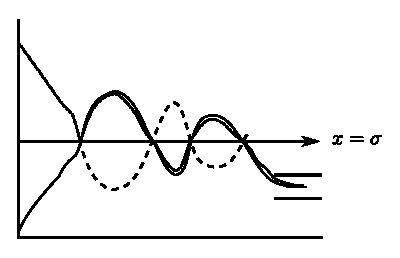
\includegraphics{figure/fig6.eps}
\end{figure}
\end{proof}

The reflection principle (or the strong Markov property) allows us to
replace this path by the dotted path (see Fig.). The symmetry of the
Brownian motion can then be used to reflect this path about the line
$x=a$ and obtain the path shown in dark. Thus we have the following
result:

{\em the probability that a Brownian particle starts from $x=0$ at
  $t=0$ and reaches $A$ at time $t$ after it has hit $x=a$ at some
  time $\tau\leq t$ is the same as if the particle started at time
  $t=0$ at $x=2a$ and reached $A$ at time $t$. (The continuity of the
  path ensures that at some time $\tau\leq t$, this particle has to
  hit $x=a$).}

We\pageoriginale shall use the intuitive approach in what follows, the
mathematical analysis being clear, thorugh lengthy.

\begin{theorem*}
Let $X(t)$ be a one-dimensional Brownian motion, $A\subset (-1,1)$ any
Borel subset of $\mathbb{R}$. Then
$$
P_{0}\left[\sup\limits_{0\leq s\leq t}|X(s)|<1, X(t)\in
  A\right]=\int\limits_{A}\phi(t,y)dy, 
$$
where
$$
\phi(t,y)=\sum\limits^{\infty}_{n=-\infty}(-1)^{n}/\surd(2\pi
t)e^{-(y-2n)^{2}/2t}.
$$
\end{theorem*}

\eject

\begin{proof}
~

\begin{figure}[H]
\centering
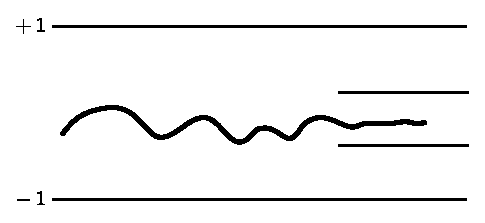
\includegraphics{figure/fig7.eps}
\end{figure}

Let $E_{n}$ be the set of those trajections which (i) start at $x=0$
at time $t=0$ (ii) hit $x=+1$ at some time $\tau_{1}<t$ (iii) hit
$x=-1$ at some later time $\tau_{2}<t$ (iv) hit $x=1$ again at a later
time $\tau_{3}<t\ldots$ and finally reach $A$ at time $t$. The number
of $\tau$'s should be equal to $n$ at least, i.e.
$$
E_{n}=\{w:\text{~ there exists a sequence~ }
\tau_{1},\ldots\tau_{n}\text{~ of}
$$
stopping times such that $0<\tau_{1}<\tau_{2}<\ldots<t_{\tau_n}<t$,
$X(\tau_{j})=(-1)^{j-1}$, $X(t)\in A\}$. Similarly, let 
\begin{align*}
F_{n} &= \{w:\text{~ there exists a sequence~
}\tau_{1},\ldots,\tau_{n}\text{~ of stopping times}\\
&\q 0<\tau_{1}<\tau_{2}<\ldots<\tau_{n}<t,X(\tau_{j})=(-1)^{j},X(t)\in A\}
\end{align*}

Note\pageoriginale that
\begin{align*}
& E_{1}\supset E_{2}\supset E_{3}\supset \ldots,\\
& F_{1}\supset F_{2}\supset F_{3}\supset \ldots,\\
& F_{n}\supset E_{n+1};\ E_{n}\supset F_{n+1},\\
& E_{n}\cap F_{n}=E_{n+1}\cup F_{n+1}.
\end{align*}

Let
$$
\phi(t,A)=P\left[\sup\limits_{0\leq s\leq t}|X(s)|<1,X(t)\in A\right].
$$

Therefore
\begin{align*}
\phi(t,A) &= P[X(t)\in A]-P\left[\sup\limits_{0\leq s\leq t}|X(s)|\geq
  1,X(t)\in A\right]\\
&= \int\limits_{A}1/\surd(2\pi t)e^{-y^{2}/2t}dy-P[(E_{1}\cup
  F_{1})\cap A_{0}],
\end{align*}
where 
$$
A_{0}=\{X(t)\in A\}=\int\limits_{A}1/\surd(2\pi
t)e^{-y^{2}/2t}dy-P[(E_{1}\cap A_{0})\cup (F_{1}\cap A_{0})].
$$

Use the fact that $P[A\cup B]=P(A)+P(B)-P(A\cap B)$ to get
$$
\phi(t,A)=\int\limits_{A}1/\surd(2\pi t)e^{-y^{2}/2t}dy-P[E_{1}\cap
  A_{0}]-P[F_{1}\cap A_{0}]+P[E_{1}\cap F_{1}\cap A_{0}],
$$
as $E_{1}\cap F_{1}=E_{2}\cup F_{2}$. Proceeding successively we
finally get
$$
\phi(t,A)=\int\limits_{A}1/\surd(2\pi
t)e^{-y^{2}/2t}dy+\sum\limits^{\infty}_{n=1}(-1)^{n}P[E_{n}\cap
  A_{0}]+\sum\limits^{\infty}_{n=1}(-1)^{n}P[F_{n}\cap A_{0}]
$$

We shall obtain the expression for $P(E_{1}\cap A_{0})$ and
$P[E_{2}\cap A_{0}]$, the other terms can be obtained similarly.

$E_{1}\cap A_{0}$ consists of those trajectries that hit $x=\pm 1$ at
some time $\tau\leq t$ and then reach $A$ at time $t$. Thus
$P[E_{1}\cap A_{0}]$ is given by the previous theorem by
$$
\int\limits_{A}1/\surd(2\pi t)e^{-(y-2)^{2}/2t}dy.
$$\pageoriginale
$E_{2}\cap A_{0}$ consists of those trajectories that hit $x=\pm 1$ at
time $\tau_{1}$, hit $x=-1$ at time $\tau_{2}$ and reach $A$ at time
$t(\tau_{1}<\tau_{2}<t)$.

According to the previous theorem we can reflect the trajectory upto
$\tau_{2}$ about $x=-1$ so that $P(E_{2}\cap A_{0})$ is the same as if
the particle starts at $x=-2$ at time $t=0$, hits $x=-3$ at time
$\tau_{1}$ and ends up in $A$ at time $t$. We can now reflect the
trajectory
\begin{figure}[H]
\centering
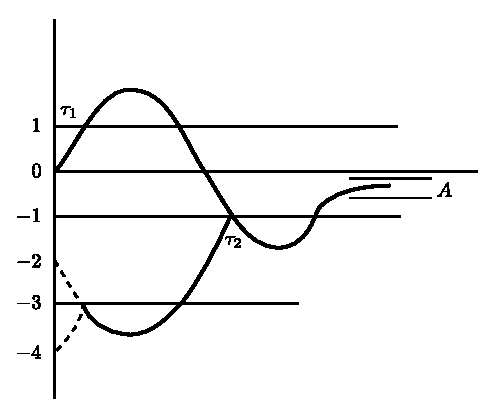
\includegraphics{figure/fig8.eps}
\end{figure}
\noindent
upto time $\tau_{1}$ (the dotted curve should be reflected) about
$x=-3$ to obtain the required probability as if the trajectory started
at $x=-4$. Thus,
$$
P(E_{2}\cap A_{0})=\int\limits_{A}e^{-(y+4)^{2}/2t/\surd(2\pi t)}dy.
$$

Thus
\begin{align*}
\phi(t,A) &=
\sum\limits^{\infty}_{n=-\infty}(-1)^{n}\int\limits_{A} 1/\sqrt{2\pi
  t}e^{-(y-2n)^{2}/2t}dy\\
&= \int\limits_{A}\phi(t,y)dy.
\end{align*}

The\pageoriginale previous theorem leads to an interesting result:
$$
P\left[\sup\limits_{0\leq s\leq
    t}|X(s)|<1\right]=\int\limits^{1}_{-1}\phi(t,y)dy 
$$

Therefore
\begin{align*}
P\left[\sup\limits_{0\leq s\leq t}|X(s)|\geq 1\right] &=
1-P\left[\sup\limits_{0\leq s\leq t}|X(s)|<1\right]\\
&= -1 -\int\limits^{1}_{-1}\phi(t,y)dy,\\
\phi(t,y)=\sum\limits^{\infty}_{n=-\infty}&(-1)^{n}/\surd(2\pi
t)e^{-(y-2n)^{2}/2t} 
\end{align*}

\medskip
\noindent
{\bf Case (i).}~ $t$ is very small.
\smallskip

In this case it is enough to consider the terms corresponding to
$n=0$, $\pm 1$ (the higher order terms are very small). As $y$ varies
from $-1$ to $1$,
$$
\phi(t,y)\simeq 1/\surd(2\pi
t)\left[e^{-y^{2}/2t}-e^{-(y-2)^{2}/2t}-e^{-(y+2)^{2}/2t}\right]. 
$$

Therefore
$$
\int\limits^{1}_{-1}\phi(t,y)dy\simeq 4/\surd(2\pi t)e^{-1/2t}.
$$

\medskip
\noindent
{\bf Case (ii).}~ $t$ is large. In this case we use Poisson's
summation formula for $\phi(t,y)$:
$$
\phi(t,y)=\sum\limits^{\infty}_{k=0}e^{-(2k+1)^{2}\pi^{2}t/8}Cos\{(k+1)/2\pi
y\},
$$
to get
$$
\int\limits^{1}_{-1}\phi(t,y)dy\simeq 4/\pi e^{-\pi^{2}t/8}
$$
for\pageoriginale large $t$. Thus, $P(\tau>t)=4/\pi e^{-\pi^{2}t/8}$.

This result says that for large values of $t$ the probability of paths
which stay between $-1$ and $+1$ is very very small and the decay rate
is governed by the factor $e^{-\pi^{2}t/8}$. This is connected with
the solution of a certain differential equation as shall be seen later
on.
\end{proof}




